\documentclass[final]{beamer}
\usetheme{SD}
\usepackage[orientation=landscape,size=custom,width=160,height=90,scale=2.2,debug]{beamerposter}
%\usepackage[absolute,overlay]{textpos}
%\setlength{\TPHorizModule}{1cm}
%\setlength{\TPVertModule}{1cm}
\usepackage{graphicx}
\usepackage{caption}
\usepackage{subcaption}

\title{Scientific Computing Interest Group}
\author{Sean Davis, Jeff Shilling, and Carl McCabe}
\footer{More information at \texttt{\url{http://bioconductor.org/}}}
\date{January 14, 2014}

\begin{document}
\begin{frame}[t]
  \begin{columns}[t]

% FIRST column
    \begin{column}{0.3\linewidth}
      \begin{block}{What is Bioconductor?}
        Bioconductor provides tools for the analysis and comprehension of high-throughput genomic data. Bioconductor uses the R statistical programming language and is open source and open development. It has two releases each year, 554 software packages, and an active user community. Bioconductor is also available as an Amazon Machine Image (AMI).
      \end{block}
      \begin{block}{Microarray Data Analysis}
        \begin{itemize}
        \item{Import Affymetrix, Illumina, Nimblegen, Agilent, and other platforms}
        \item{Microarray quality assessment, normalization, differential expression}
        \item{Clustering and classification}
        \item{Gene set enrichment and pathway analysis}
        \item{Workflows available for:}
     \begin{itemize}
       \item{Gene expression}
       \item{Exon arrays}
       \item{Copy number}
       \item{SNP}
       \item{Methylation}
     \end{itemize}
        \end{itemize}
      \end{block}
    \end{column}

% BEGIN SECOND column
    \begin{column}{0.3\linewidth}
      \begin{block}{Graphical Capabilities of Bioconductor}
        \begin{figure}
          \centering
          \begin{subfigure}{.45\textwidth}
            \centering
            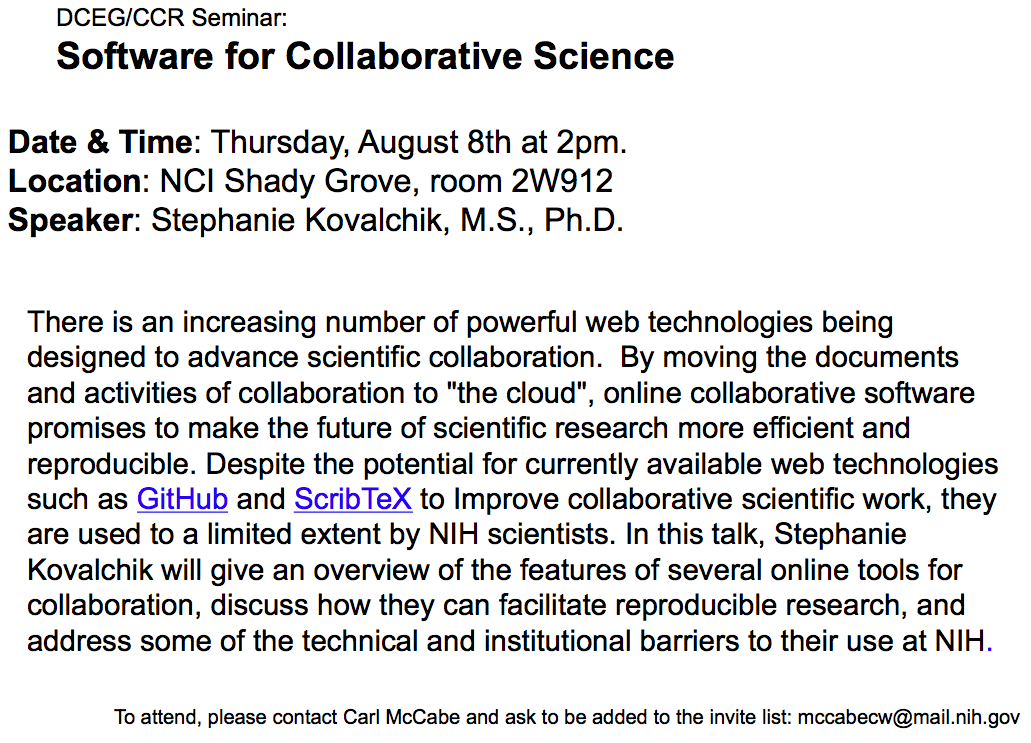
\includegraphics[width=1\linewidth]{collabSoftwareTools}
            \caption{A subfigure}
            \label{fig:sub1}
          \end{subfigure}
          \begin{subfigure}{.45\textwidth}
            \centering
            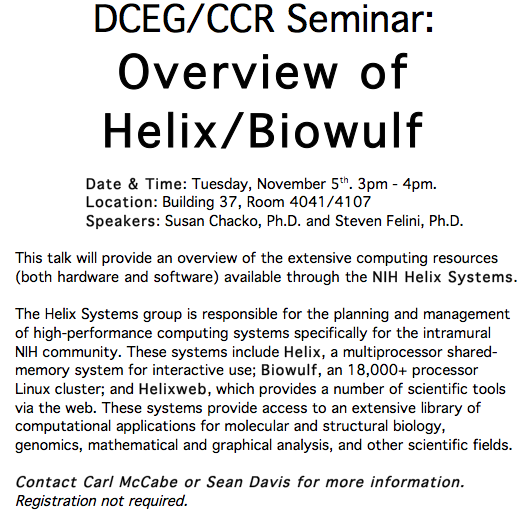
\includegraphics[width=1\linewidth]{helixOverview}
            \caption{A subfigure}
            \label{fig:sub2}
          \end{subfigure}
          \caption{A figure with two subfigures}
          \label{fig:test}
        \end{figure}
      \end{block}
    \end{column}

% BEGIN THIRD column
    \begin{column}{0.3\linewidth}
      \begin{block}{Next-Generation Sequencing Analysis}
        \begin{itemize}
          \item{Import fasta, fastq, ELAND, MAQ, BWA, Bowtie, BAM, gff, bed, wig, and other sequence formats} 
          \item{Trim, transform, align, and manipulate sequences}
          \item{Workflows}
            \begin{itemize}
              \item{Quality assessment}
              \item{ChIP-seq}
              \item{RNA-seq and differential expression}
            \end{itemize}
          \item{Access the NCBI Sequence Read Archive}
        \end{itemize}
      \end{block}
      \begin{block}{Genomic Variants}
        \begin{itemize}
          \item{Read and write VCF files}
          \item{Identify coding variants}
          \item{Use SIFT and PolyPhen to annotate variants}
          \item{Overlap variants with arbitrary genomic annotations}
        \end{itemize}
      \end{block}
      \begin{block}{Data Integration}
        Use of consistent data structures in the R statistical computing environment allows for complex data integration and multi-assay hypothesis generation and testing.
      \end{block}
    \end{column}
    \end{columns}
  \end{frame}
\end{document}
